%%%%%%%%%%%%%%%%%%%%%%%%%%%%%%%%%%%%%%%%%%%%%%%%%%%%%%%%%%%%%%%%%%%%%%%
% Based on IEEE the conference template available                     %
% at https://www.ieee.org/conferences/publishing/templates.html       %
% Adapted for the Data Science Lab course at Politecnico di Torino    %
% by Giuseppe Attanasio, Flavio Giobergia                             %
% 2020, DataBase and Data Mining Group                                %
%%%%%%%%%%%%%%%%%%%%%%%%%%%%%%%%%%%%%%%%%%%%%%%%%%%%%%%%%%%%%%%%%%%%%%%

\documentclass[conference]{IEEEtran}
\usepackage{cite}
\usepackage{amsmath,amssymb,amsfonts}
\usepackage{algorithmic}
\usepackage{graphicx}
\usepackage{textcomp}
\usepackage{xcolor}


\begin{document}

\title{Estimating the age of people from vocal recordings}

\author{\IEEEauthorblockN{ Bello Renato}
\IEEEauthorblockA{\textit{Politecnico di Torino} \\
Student id: s341965 \\
s341965@studenti.polito.it}
\and
\IEEEauthorblockN{Chiodo Martina}
\IEEEauthorblockA{\textit{Politecnico di Torino} \\
Student id: s343310 \\
s343310@studenti.polito.it}
}

\maketitle

\begin{abstract}
In this report we tried to solve a regression problem, the goal is to estimate the age of a person from a vocal recording. We used both the csv dataset and the vocal recording to extract all the features needed to make the regression.
\end{abstract}

\section{Problem overview}
% Here you should describe your problem
The proposed competition is a regression problem about age estimating, in fact based on vocal recordings and some informatoon regarding the person, such as his ethnicity and his gender, we aim to correctly determine the age of the person who is talking.
The dataset is divided in two parts:
\begin{itemize}
    \item a \emph{development} set, containing $2933$ elements, each of them labeled  
    \item an \emph{evaluation} set, containing $691$ elements
\end{itemize}
The development set will be used to build a regressor to label the elements of the evaluation set.

We can make some considerations based on the development set. First, the dataset is complete, indeed non of the rows contains missing values. 
Second, some features requires some preprocessing: \emph{ethnicity} and \emph{gender} are a categorial features and, thus, they need to be encoded in order to be used in the regression; \emph{tempo} is not automatically saved as a float type because the values are enclosed by parenthesis.
Third, the dataset also contains the path to the vocal recordings from which we have decided to extract more features from the spectogram.

We can study the correlation of the feature given by the dataset by analizing the correlation plot shown in figure $\eqref{correlation_plot}$.
\begin{figure}
    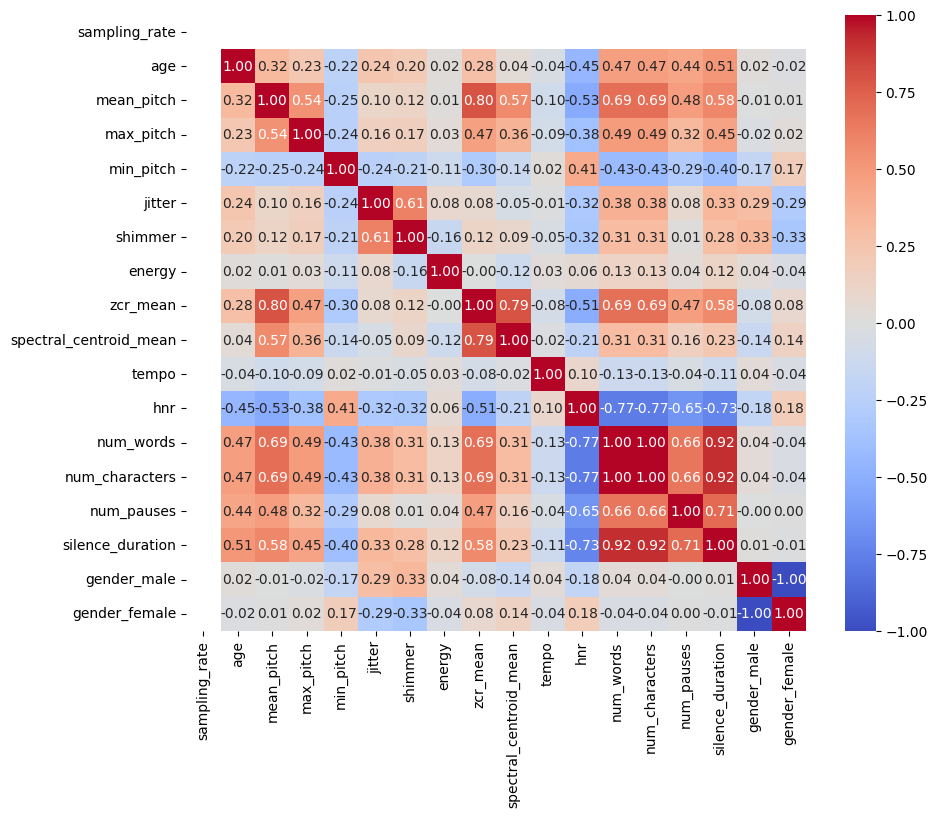
\includegraphics[width = 0.47\textwidth]{img/correlation_plot.png}
    \caption{Correlation among features.}
    \label{correlation_plot}
\end{figure}

To better understand the distribution of the features we can plot some histograms.
From the histograms shown in figure $\eqref{hist_distributivi}$ we can notice that most of the features seems to be distributed as Gaussian distribution with not many outliers. 
Some exceptions are \textit{max\_pitch}, \textit{min\_pitch} and \textit{num\_characters}: the first two features mentioned have a very wide range of values but almost all their distribution mass is concentrated in a single point, thus there are many outliers; on the contrary, \textit{num\_characters} concentrates his mass distribution in two far values.

\begin{figure}
    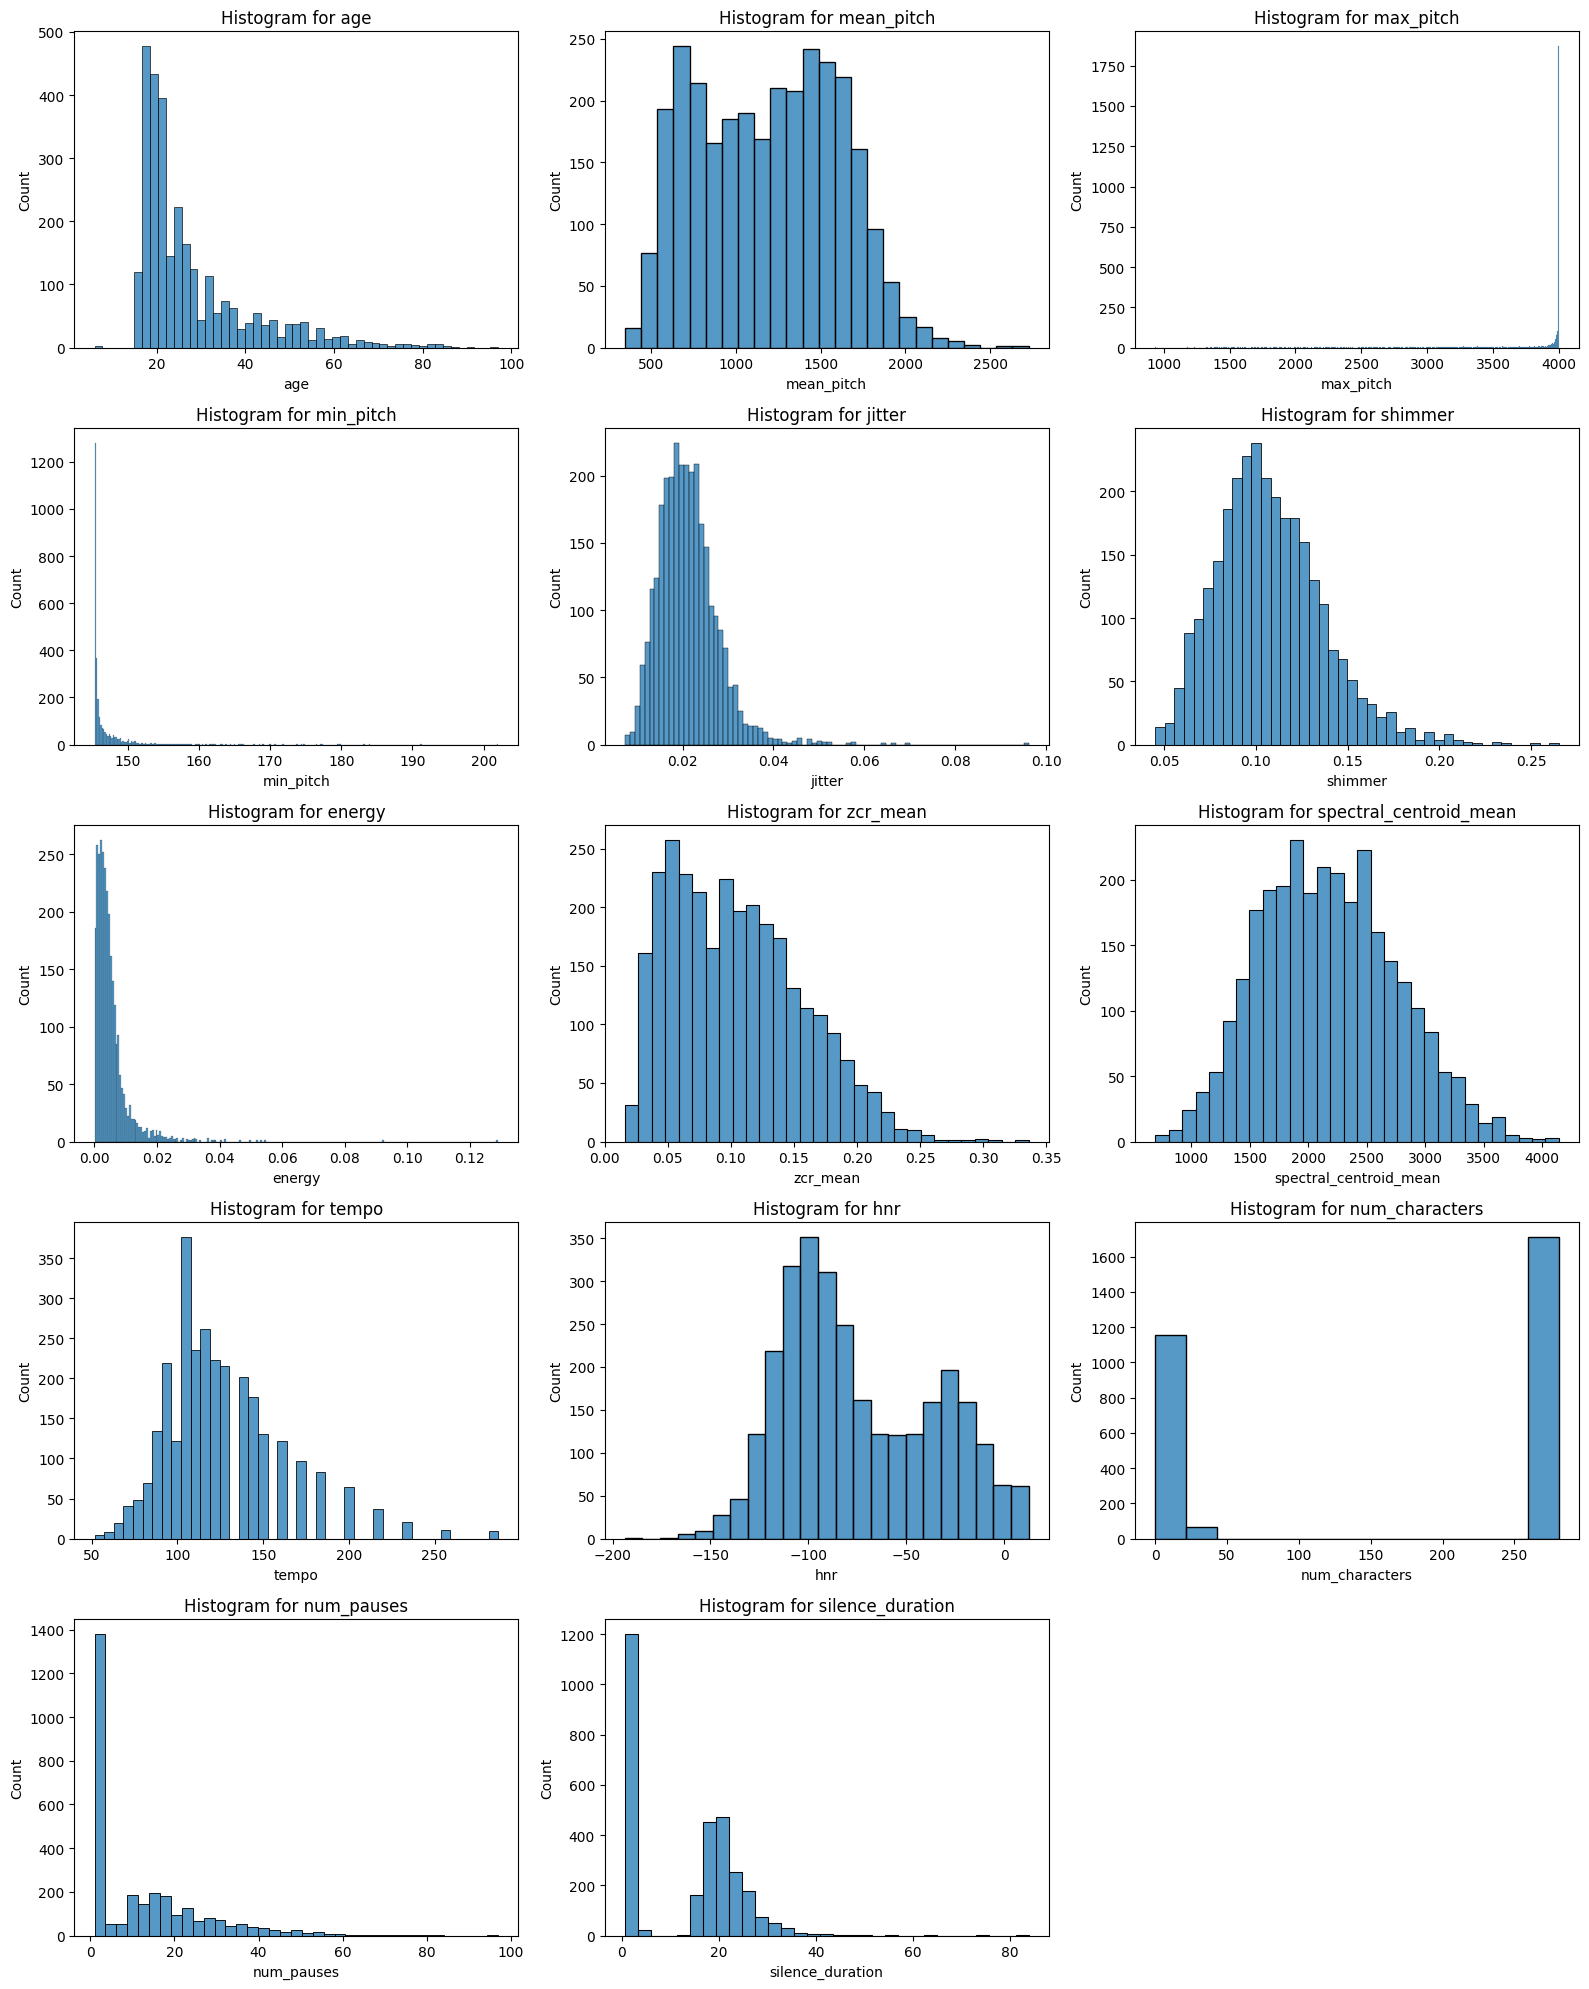
\includegraphics[width = 0.47\textwidth]{img/distribuzioni_features.png}
    \caption{Histograms of some features.}
    \label{hist_distributivi}
\end{figure}

\section{Proposed approach}
% In this section, you will present your solution. Please fill in accordingly.
\subsection{Preprocessing}
er sfruttare sia il dominio temporale che quello di frequenza, utilizziamo gli spettri di ogni segnale. ...
\subsection{Model selection}
We choose 2 models for testing our regression. 
\begin{itemize}
    \item \textit{Ridge regression}\cite{Ridge}: is a particular linear regression where the objective function to minimize is defined as: 
    \begin{equation}
        \mathcal{L}(\mathbf{w})=\frac{1}{n}\sum_{i=1}^n\left(y_i - \mathbf{x}_i^\top\mathbf{w} \right) + \lambda\| \mathbf{w}\|_2^2
    \end{equation}
    Where \(y_i\) is the target variable, \(\mathbf{x}_i\) are the characteristics and \(\mathbf{w}\) are the coefficients of the regression. Instead of the classical linear regression, in this function there is a term (\(\lambda\|\mathbf{w}\|_2^2\)) that imposes a penalty proportional to the squared \(L_2\)
    norm of the coefficients to encourage the reduction of their overall magnitude.
    \item \textit{MLP regression}\cite{MLP}: this regression id based on a \textit{neural network} that uses the \textit{MSE} \eqref{MSE} (\textit{mean squared error}) as a \textit{loss function}, which is minimized using a stochastic gradient method and the \textit{backpropagation}.
    \begin{equation} \label{MSE}
        MSE = \frac{1}{n}\sum_{i=1}^n\left(y_i-\hat{y}_i\right)^2
    \end{equation}
    In this formula \(\hat{y}_i\) represents the prediction made by the neural network for the target variable \(y_i\).
\end{itemize}
For both classifiers, the best working configuration of hyperparameters has been identified through a grid search, as explained in the following sections.
\subsection{Hyperparameter tuning}
There are two main sets of hyper-parameters to be tuned:
\begin{itemize}
    \item The number of features to use to fit each model is indicated by $n_{RI}$ and $n_{MLP}$.
    \item Ridge regressor and MLP regressor parameters
\end{itemize}
For tuning the parameters we considered a split of the development set into \textit{train} and \textit{validation} set, containing the 80\% and the 20\% of the points.

For convenience we assume that two set are independent, therefore we can first optimize the number of features used to fit the regressor and then perform some tuning of the hyper-parameters of the two regressor.

\begin{itemize}
    \item \textit{Ridge parameters}: Before finding the best parameters using a grid search, we found the best features for fitting the regression. We used a \textit{scikit-learn} class called \textit{RFE}\cite{RFE} (\textit{recursive features elimination}), to execute this task. We trained and tested the ridge model increasing the feasible number of features each time, obtaining that the best number of features is 50, as shown in Figure \ref{num vs rmse}. The feature selection has been performed by using the default parameters.
    \begin{figure}
    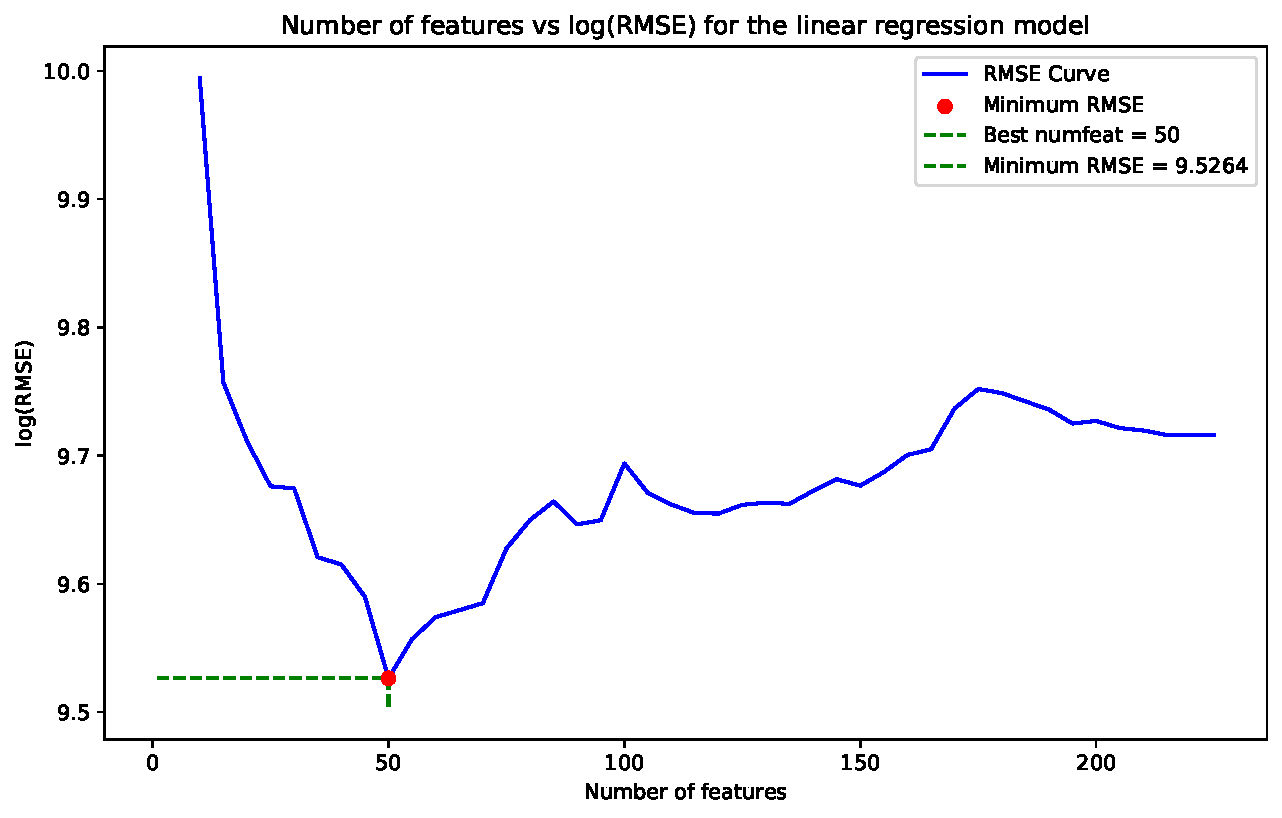
\includegraphics[width = 0.40\textwidth]{img/rmse_curve_linear_2.pdf}
    \caption{number of features vs log(RMSE) for the Ridge regression}
    \label{num vs rmse}
    
\end{figure}


\item \textit{MLP parameters}: Before finding the best parameters using a grid search, we found the best features for fitting the regression. For the \textit{MLP regressor} we used a \textit{scikit-learn} class called \textit{SelectKbest}\cite{SelectKbest}, to execute this task. We trained and tested the \textit{MLP regressor} increasing the feasible number of features each time, obtaining that the the best number of feature for fitting the regression is 40, as shown in Figure \ref{num vs rmse MLP}. The feature selection has been performed using, as initial guess for the MLP Regressor, the following parameters: \textit{hidden\_layer\_sizes} = (50,), \textit{activation} = \textit{relu}, \textit{alpha} = 0.01 and \textit{max\_iter} = 2000.

\begin{figure}
    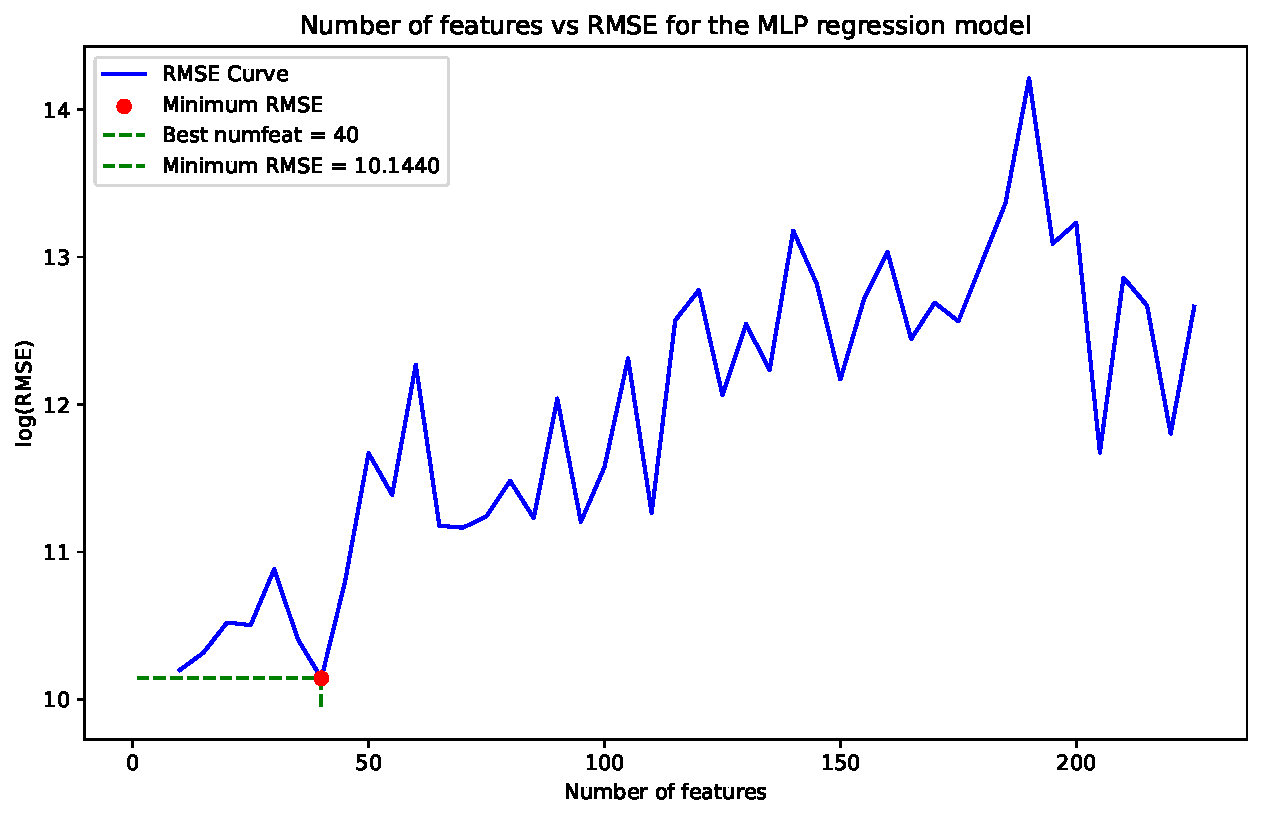
\includegraphics[width = 0.40\textwidth]{img/rmse_mlp_new.pdf}
    \caption{number of features vs log(RMSE) for the MLP regression}
    \label{num vs rmse MLP}
    
\end{figure}

\end{itemize}

After finding the best features for the two models, we applied a grid search for finding the best hyper-parameters, those are shown in the table \ref{tab:hyperparameters}. 

We incorporated the grid search with a 5-fold cross-validation, to ensure greater model robustness. The parameters have been selected by choosing the ones which minimized the mean squared error.

\begin{table}[ht]
    \centering
    \caption{Hyperparameters considered for the grid-search ($n_{tot}$ is the total number of features)}
    \begin{tabular}{@{}lll@{}}
        \toprule
        \textbf{Model} & \textbf{Parameter} & \textbf{Values} \\ \midrule
        Feature Selection & $n_{RI},  n_{MLP}$ & $10
        \to n_{tot}$, step $5$ \\ \midrule
        \multirow{3}{*}{Ridge Regressor} 
            & alpha & \{0.5, 1, 2\} \\
            & fit\_intercept & \{True, False\} \\
            & max\_iter & \{None, 500, 1000\} \\ \midrule
        \multirow{2}{*}{MLP Regressor} 
            & hidden\_layer\_sizes & \{(100,), (100,2), (50,)\} \\
            & activation & \{tanh, logistic, relu\}\\
            & solver & \{adam, lbfgs, sgd\} \\
            & alpha & \{0.001, 0.01, 1\} \\
            & max\_iter & \{1000, 2000\} \\ \bottomrule
    \end{tabular}
    \label{tab:hyperparameters}
\end{table}



You can use citations as follows: \cite{goodfellow2016deep} (you can add BibTeX citations in the \textit{bibliography.bib} file).


\section{Results}
% Here you will present your results (models \& configurations selected, performance achieved)
From applying the pipeline we have just discussed, we obtained the following hyper-parameters for Ridge Regressor
\begin{itemize}
    \item $n_{RI} = 50$
    \item \textit{alpha}: 2
    \item \textit{fit\_intercept}: \textit{True}
    \item \textit{max\_iter}: \textit{None}
\end{itemize}
while for the MLP Regressor the hyper-parameters are
\begin{itemize}
    \item $n_{MLP} = 40$
    \item \textit{hidden\_layer\_sizes}: (100,)
    \item \textit{activation}: \textit{logistic}
    \item \textit{solver}: \textit{adam}
    \item \textit{alpha}: 1
    \item \textit{max\_iter}: 1000
\end{itemize}


Once defined the quantities $n_{RI}$ and $n_{MLP}$ and tuned the hyper-parameters using a portion of the development set, we validated the resultant regressors on the other part of the dataset.

A first analysis of the performance of the model can be done by looking at the residuals, that is the quantity $\epsilon_i = y_i - \hat{y_i}$. 
Theoretically, they should represent the white noise in data and thus should be distributed as
$$\epsilon_i \overset{\text{iid}}{\sim} \mathcal{N}(0, \sigma^2)$$

Looking at the behaviour of the residuals we obtained, shown in \eqref{fig:res_Ridge} and \eqref{fig:res_MLP}, we can appreciate that they are distributed around the mean value 0 for both models, but the hypothesis of homoscedasticity is not satisfied. The cause could be a lacking representativeness of people over the age of 50 in the dataset, as noticed during the data exploration and confirmed by the fact that most of the residuals are positive, meaning that the two regressors often predict a smaller age when the true one is over 35.

Moreover, we sadly notice that the variance of the residuals is very large especially when predicting larger values of the response variable. Comparing the two plots, it has to be said that the MLP regressor is the one whose residuals have greater variance.

\begin{figure}
    \centering
    % First PDF image
    \begin{subfigure}{0.23\textwidth}
        \centering
        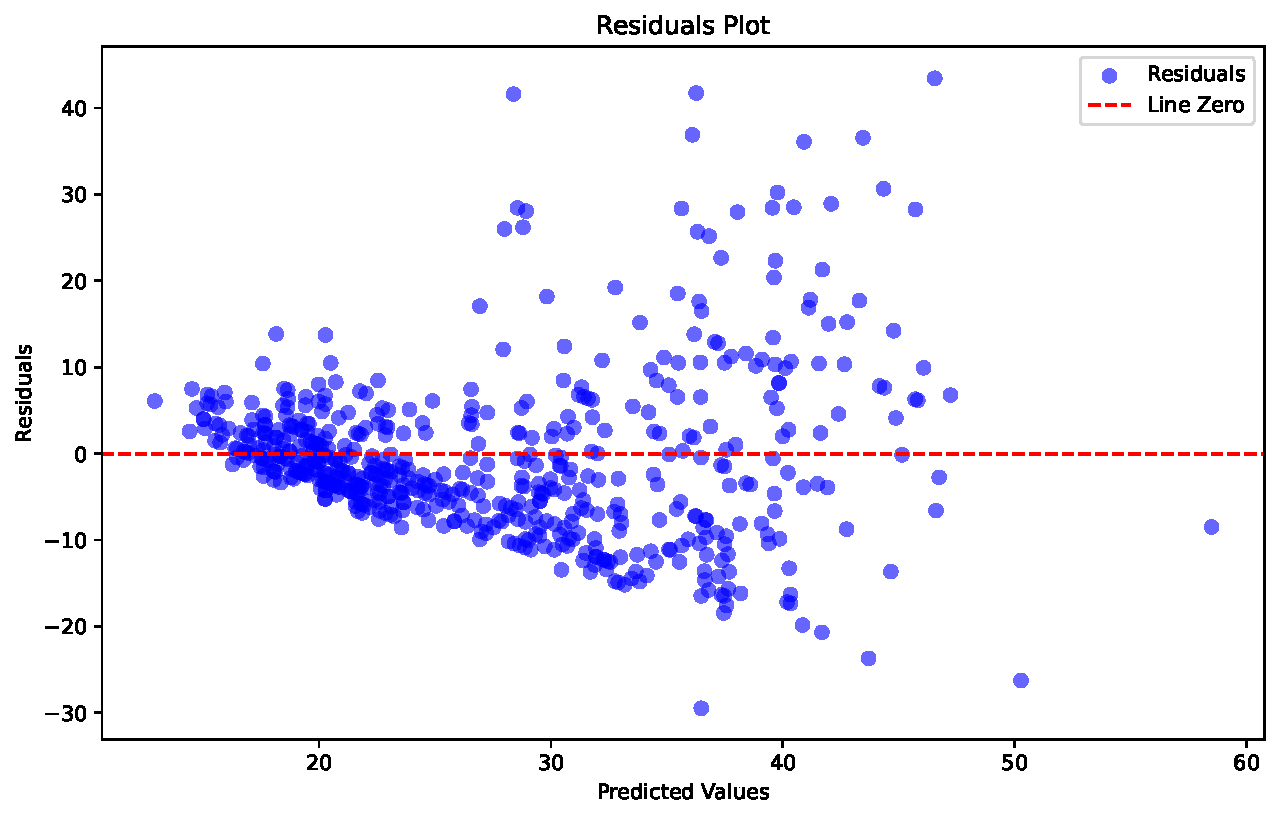
\includegraphics[width=\textwidth]{img/residuals_RI_1.pdf}
    \end{subfigure}
    % Second PDF image
    \begin{subfigure}{0.23\textwidth}
        \centering
        
\includegraphics[width=\textwidth]{img/residuals_RI_2.pdf} 
    \end{subfigure}
    \caption{Residuals plot and distribution for the Ridge Regressor}
    \label{fig:res_Ridge}
\end{figure}

\begin{figure}
    \centering
    % First PDF image
    \begin{subfigure}{0.23\textwidth}
        \centering
        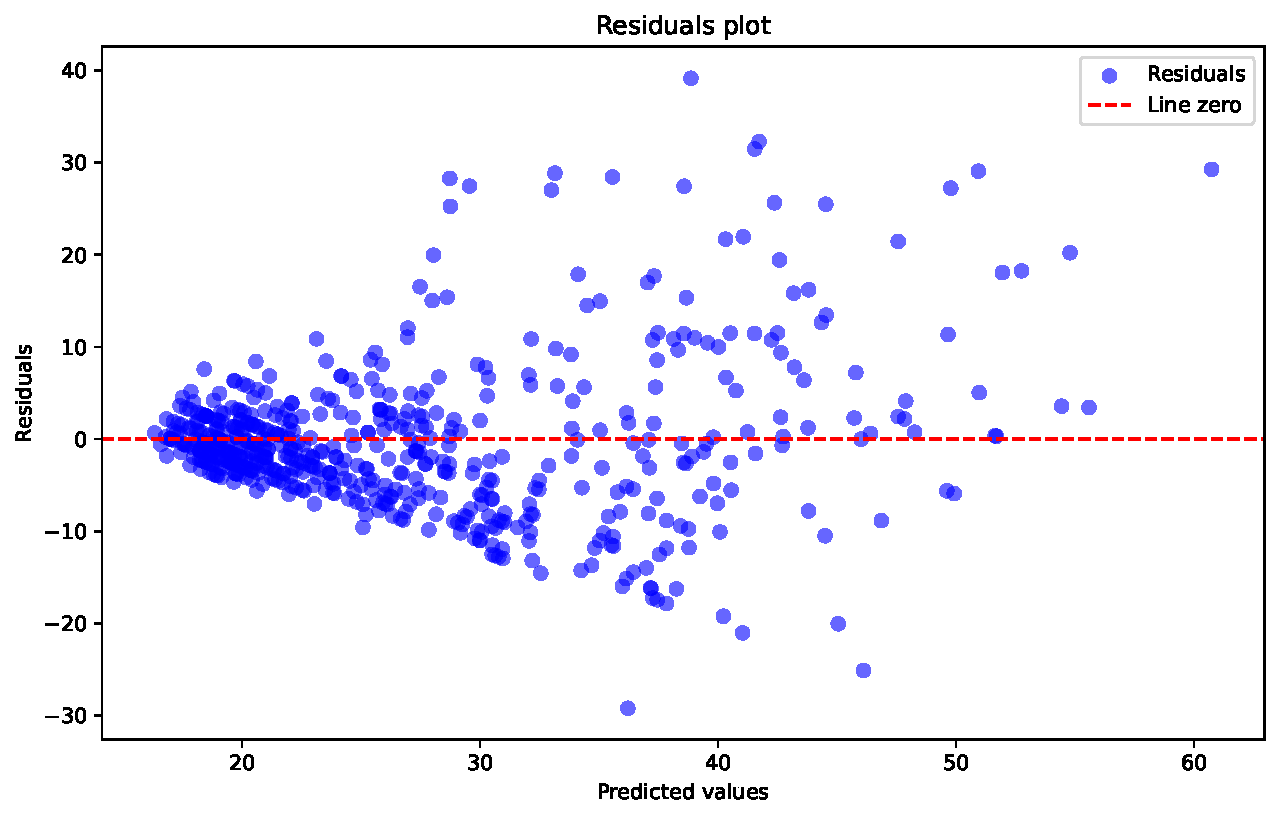
\includegraphics[width=\textwidth]{img/residuals_mlp_2.pdf}
    \end{subfigure}
    % Second PDF image
    \begin{subfigure}{0.23\textwidth}
        \centering
        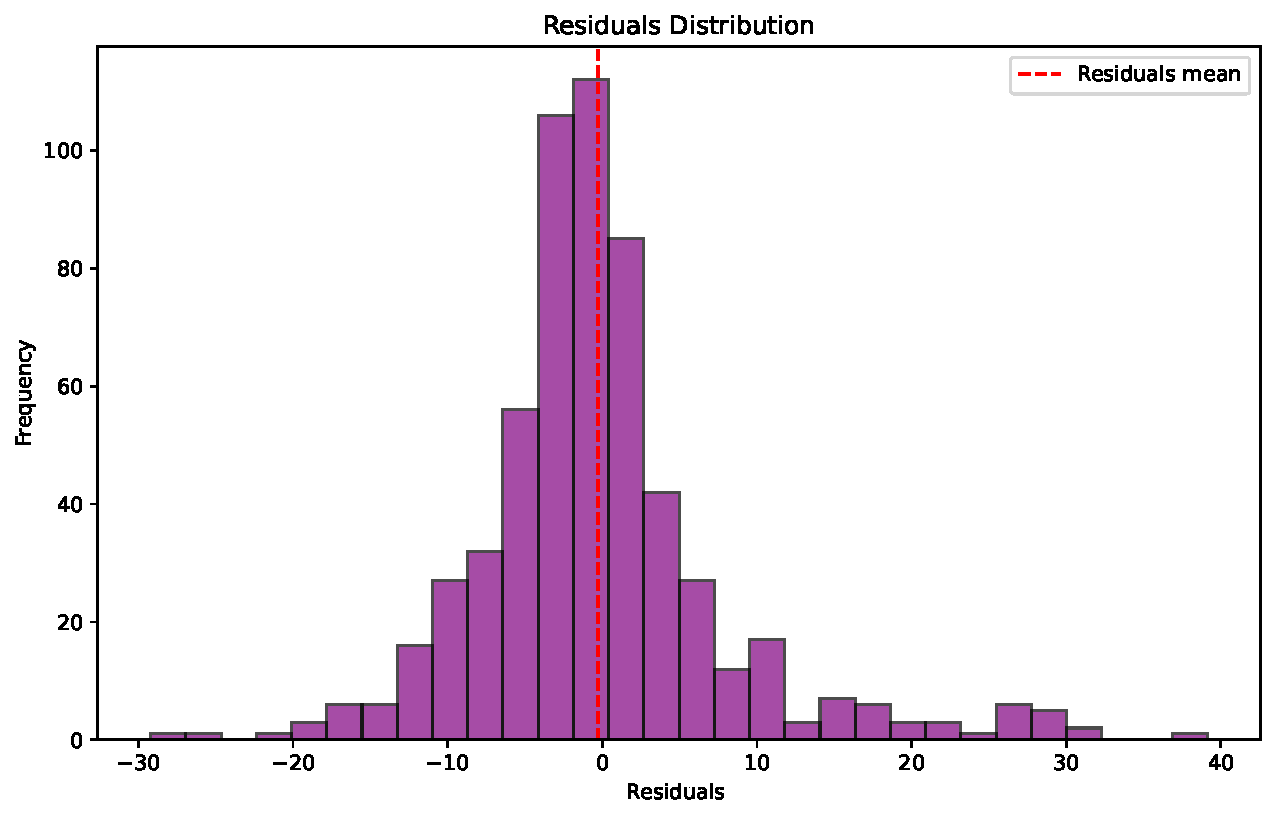
\includegraphics[width=\textwidth]{img/residuals_mlp_1.pdf} 
    \end{subfigure}
    \caption{Residuals plot and distribution for the MLP Regressor}
    \label{fig:res_MLP}
\end{figure}

During the phase of validation, we decided to evaluate the model not only in terms of RMSE but also by computing the $R^2$ score: the scores obtained are of 0.4520 for the Ridge regressor and of 0.3927 for the MLP regressor. The fact that the MLP Regressor is scored with a lower $R^2$ value restates what was shown in the residuals plots, that is that the MLP regressor residuals have higher variance.
This allows us to say that the solution we have found works slightly better than just predicting the mean value of the response variable. Still, they are pretty far from their maximum value 1 which means that the regressors fail to capture great part of the variance of the data.

The public score obtained is 9.974 for the Ridge Regressor and 9.726 for the MLP Regressor.
As these represent the first scores derived from the evaluation data, overfitting is unlikely, and it is reasonable to expect similar results on the private score.

\section{Discussion}
% Any relevant discussion goes here.
\input{chap/discussions.tex}


\bibliography{bibliography}
\bibliographystyle{ieeetr}

\end{document}
